\section{Infrastructure Support}

This section discusses miscellaneous aspects related to Lustre initialization,
client registration, obd devices management, etc.

\subsection{Lustre Client Registration}

Lustre client side or Lustre Lite registers as a filesystem with the name
``lustre.''  The file system type is defined as:

\begin{Verbatim}
    struct file_system_type lustre_fs_type = {
        .owner      = THIS_MODULE,
        .name       = "lustre",
        .get_sb     = lustre_get_sb,
        .kill_sb    = lustre_kill_super,
        .fs_flags   = FS_BINRARY_MOUNTDATA | FS_REQUIRES_DEV 
                        LL_RENAME_DOES_D_MOVE,
    };
\end{Verbatim}

Another function defined by \url{lustre_register_fs()} simply invokes kernel
function:

\begin{Verbatim}
    return register_filesystem(&lustre_fs_type);
\end{Verbatim}

and will be done with the registration. This was invoked when \url{obdclass} as
a module was being initialized.
 
\begin{Verbatim}
int init_obdclass(void) {
...
#ifdef __KERNEL__
    err = lustre_register_fs()
#endif
}
\end{Verbatim}

See \url{class_obd.c} for more details.

\subsection{Superblock and Inode Registration} 

It should be a relatively simple matter, but Lustre jumps through several hoops
that may be due to some legacy support issues.

When Lustre Lite initializes as a Linux module, \url{init_luster_lite()} was
defined in \url{super25.c} \footnote{It is actually used for Linux Kernel 2.6 as well.} 
Among things such as allocating inode cache, it assigns (essentially)
the function pointer \url{*client_fill_super} with \url{ll_fill_super}.

In the \url{luster_fill_super()} method, we check if this is a client mount.
If it is, it makes calls to \url{(*client_fill_super)(sb)}, where \url{sb} is
the superblock.


\subsection{OBD Device}

OBD device is meant to provide a level of abstraction on Lustre components such
that the generic operations can be applied without knowing the specific devices
you are dealing with. We discussed the method tables defined on it in Section
\ref{sec:ost-and-obdfilter}. Lustre also provides some generic infrastructure
for managing object devices. The core structures are \url{obd_devices} and
\url{exports}. We discuss them in detail.

Each obd device was assigned an integer number, there are at most
\url{MAX_OBD_DEVICES} obd devices that can be created on a given node. You can retrieve an
obd device through an integer number (\url{obd_minor}), a name, or a uuid. All obd
devices are stored in an array internally. However, the preferred way to
retrieve an obd device is through a set of API as discussed below.

\begin{comment}
OBD device can be clustered into a group, in that case, they will share
a common group id.
\end{comment}

\begin{Verbatim}
struct obd_device *obd_devs[MAX_OBD_DEVICES]
\end{Verbatim}

The API can be roughly divided into five categories:

\begin{itemize}

\item Register and unregister a device type.

\item Allocate and free obd devices. \url{obd_device_alloc()},
\url{obd_device_free()}.


\item Create and release obd devices. You can create new obd devices
by giving a string type and string name through \url{class_newdev()}. 
You can release one by giving a pointer to \url{obd_device} that it is to be
released. In both cases, they internally invoke allocation and free
functions.

\item Search. You can search by type through \url{class_search_type()}; 

\item Conversion utilities.

\end{itemize}


\subsection{Import and Export}

For two OBD devices $A$ and $B$ to communicate, they need an import and export
pair: $A_{import}$ and $B_{export}$. $A_{import}$ is for sending requests and
receiving replies, and $B_{export}$ is for receiving requests and sending
replies.  However, the same pair cannot be used the other way around: that is 
you cannot send a request through $B_{export}$. For that to happen, such as in
the case of sending ASTs, you need so-called ``reverse import.'' Essentially,
reverse import converts the $A_{import}$ and $B_{export}$ pair into an $A_{export}$
and $B_{import}$ pair. The need for establishing such a pair at OBD
devices is partially illustrated in Figure \ref{fig:exp}.


\begin{figure}[htb]
\centering
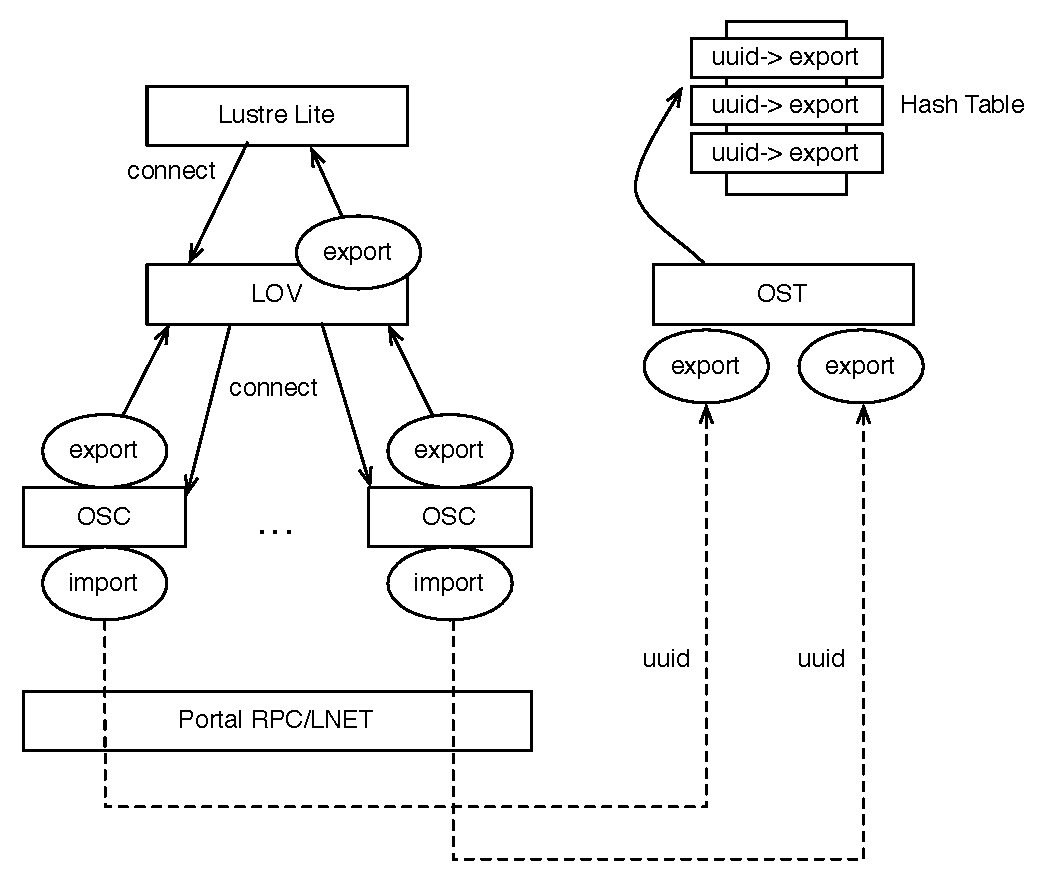
\includegraphics[width=4.5in]{img/lustre_exp}
\caption{Setup export and import.}
\label{fig:exp}
\end{figure}

Note that LOV, OSC, and OST in the figure are all defined as types of OBD
devices.

%%%%%% this figure is kinda of duplicate of above one 
%%%%%%
\begin{comment}

\begin{figure}[hbt]
\centering
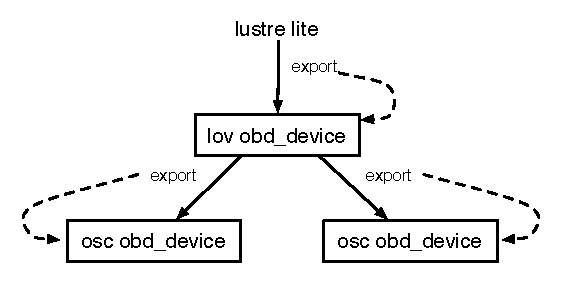
\includegraphics[width=3in]{img/exports}
\end{figure}

\end{comment}


\begin{comment}
\section{Debugging Lustre}

\subsection{Tracing}

We can learn the call sequences by turning on all debug traces of
Lustre. The following steps detail how by looking at a simple touch
operation.

\begin{Verbatim}
ictl    clear                       # clear previous log
echo -1 > /proc/sys/lnet/debug      # turn on all debugs
touch /mnt/lustre/fwang2.img
lctl dk > /tmp/touch.trace          # dk -> dump kernel
\end{Verbatim}

\end{comment}
